% INNAN DU COMMITAR!
% Uppdatera datum
% Uppdatera version
%-----
% Document name

\documentclass[10pt,a4paper]{article}
\usepackage[utf8]{inputenc}
\usepackage[english]{babel}
\usepackage{amsmath}
\usepackage{amsfonts}
\usepackage{amssymb}
\usepackage{graphicx}
\usepackage{geometry}
\usepackage{enumitem}
\usepackage{titlesec}
\usepackage{placeins}
\usepackage{subcaption}
\newcommand{\tsss}{\thesubsubsection}

\title{PostCardBuddy}
\author{Team C}

\setcounter{secnumdepth}{4}

\titleformat{\paragraph}
{\normalfont\normalsize\bfseries}{\theparagraph}{1em}{}
\titlespacing*{\paragraph}
{0pt}{3.25ex plus 1ex minus .2ex}{1.5ex plus .2ex}


\begin{document}
\begin{titlepage}
\newgeometry{left=2cm,top=1cm,right=2cm}
\newcommand{\HRule}{\rule{\linewidth}{0.5mm}}


\begin{flushright}
December 10, 2015 v2.04\\[3cm]
\end{flushright}


\centering
\textsc{\LARGE Team C}\\[0.5cm]

\HRule \\[0.4cm]
{ \huge \bfseries PostCardBuddy}\\[0.3cm]
{\Large \bfseries System Requirements}\\[0.4cm] % Title of your document
\HRule \\[1.5cm]

\vfill
\begin{flushleft}
\textit{Authors of this document:}\\
Emma Albertz\\
Caroline Brandberg\\
Linnéa Claesson\\
Billy Johansson\\
Johan Ju\\
Jacob Mejvik\\
Carl Rynegardh
\end{flushleft}

\end{titlepage}
\pagenumbering{gobble}



%\begin{center}
%\textit{\large Version History}
%
%    \begin{tabular}{ | l | l | l | p{5cm} |}
%    \hline
%    \textbf{Version} & \textbf{Date} & \textbf{Responsible} & \textbf{Description} \\ \hline
%    1.0 & 2015-10-14 & EA, LC & Baseline\\ \hline
%    \end{tabular}
%\end{center}



\setcounter{tocdepth}{2}
\tableofcontents
\newpage
\pagenumbering{arabic}

%-------------------------------------------------------------------%
%---------------------- Introduction -------------------------------%
%-------------------------------------------------------------------%
\section{Introduction}
This document is written within the context of the course Requirements Engineering at Lund Institute of Technology, which the authors are currently enrolled in. The authors have been provided with a project mission from another group, specifying a product they want to see developed. This group has also acted as the key customer. The intention of this document is to specify the requirements of this product, namely PostCardBuddy.


%-------------------------------------------------------------------%
%---------------------- Background ---------------------------------%
%-------------------------------------------------------------------%
% Extend background from PMv2
\section{Background}
The process of sending postcards is time consuming and somewhat tedious. The product described in this document aims to solve this problem by providing an easy and efficient way to send personalized postcards directly from a smart phone. Simply choose an image for the front of the postcard, add a greeting on the back and send it to your friends and family. The image for the front can be a photo to capture a moment, an image from the phone's gallery or a template image. The template images can be found in the applications standard gallery. When the user presses the send button in the application the postcard is sent to a printer. The postcard is then delivered to the postal service for further forwarding to the final recipient. 

%Everybody likes receiving postcards, but the process of sending them is tedious and takes too much effort. This is what PostCardBuddy hopes to change. PostCardBuddy is a mobile application that will simplify the process, whether you want to be creative and design your own postcards or make it easy for yourself and use a template postcard based on your location and send it to everyone in your contact list. 
%
%The application is perfect for every occasion you want to send a postcard. Grandma's birthday is coming up? Send a postcard of you and your cousins! Christmas is around the corner? Send everyone in your contact list a postcard of your cats! Away on vacation? Why not send a ready-made postcard that shows off the amazing beach to everyone in the office? Nobody needs to know it rained all week. 
%
%PostCardBuddy is the perfect tool when you want to let someone know you are thinking of them, no matter the occasion.

%--------------------------------------------------------------------%
%----------------- System Requirements ------------------------------%
%--------------------------------------------------------------------%
% Different types of system requirements (e.g. data, function, quality) at different levels (e.g. goal, domain, product, design).
% Each requirement should have a unique identity (name or number) that is consistent between releases.
% A subset of the requirements should be prioritized.

% 3A) more than two types of requirement (e.g. data, function, quality), and more than three abstraction levels (e.g. goal, domain, product, design) 
% 4A) combine different degrees of completeness and different levels of abstraction
% 4C) provide explicit requirements rationale that reduce risks of misinterpretation.
% 4D) use hierarchies and requirements relations to manage evolving requirements structures.
% 5G) use prioritization to focus improvements of specification quality and elicitation efforts for a well motivated subset of requirements.

\section{Definitions and terms}
\begin{description}
\item [Application] The part of the product that is downloaded to the device.
\item[Device] Mobile device (e.g. smart phone) on which it is possible to download and use applications.
\item [E-card] An image and a greeting sent digitally presented to look like a physical postcard.
\item[Mobile user] Person who owns a device. 
\item[Payment service] A company who provides a payment solution for applications. 
\item[Payment solution] A feature that makes it possible to charge costumers in the application. 
\item[Personalized postcards] Postcards were the design is chosen by the person who sends the postcard. 
\item[Phone gallery] User's existing image gallery on phone.
\item [Physical postcard] A printed piece of paper with an image on the front, a greeting, recipients and postage at the back. 
\item[Postal service] A company that delivers mail to private citizens.
\item [Postcard] The representation of physical postcards or E-cards within the application. 
\item[Printer of postcards] The company who delivers the postcards from the printer to the postal service. In this project the key customer.
\item[Product]The application described in this Requirement Specification.
\item[Recipient]The person whom a postcard is addressed to.
\item[Standard gallery] Gallery of pre-existing images in the application.
\item[Supplier of images] The companies or people who supply the application with images for the standard gallery.
\item [Template Greeting] Pre-made suggestion for a greeting provided by the application. 
\item [Template Image] Images in the standard gallery. 
\end{description}

\section{System Requirements}

\subsection{Goal}
The product aims to establish the key customer in the postcard sending market and shall achieve this through the following goals:

\begin{enumerate}
\item Simplify the process of sending postcards \label{goal:simpl}
\item Enable user to send personalized postcards \label{goal:pers}
\item Enable revenue generation for the printer of postcards \label{goal:rev}
\end{enumerate}

\subsection{Functional Requirements}
This section describes the functions and features of the application.

\subsubsection{Domain}
The domain level requirements provides information about how PostCardBuddy interacts with its surroundings. 

\paragraph{Context Diagram}
The context diagram of the product can be found in figure~\ref{fig:context}. This diagram shows the environment of the product and the stakeholders interacting with it. The demarcation between the inner and outer domain is based on whether the interaction with PostcardBuddy is direct. For example the printer is in the inner domain because the developer will have to take this interface into account when constructing the product. 

There is one stakeholders that will interact directly with the application, namely the mobile user. The mobile user will use the application for creating personalized postcards. For the front of the postcard the user shall be able to select an image from the application's standard gallery. These images will be provided through an image database. The specification of the image database is out of the scope of this document. Images are provided to the database by a \textit{Supplier of images}.

Some of the features of the product will require the use of functionality already present in the the device. The camera will be used to enable the user to take a picture. The GPS will provide the location of the user. The contacts will be used to select recipients. Finally the E-mail functionality in the device will be used when sending E-cards.
 
When a user sends a physical postcard it will be sent to a printer. The  \textit{Printer of postcards} has access to the printer and delivers the postcard to the postal service.  Finally the postal service delivers the physical post card to the final recipients. \textit{Printer of postcards} is responsible for a franking agreement with the postal service.

When sending physical postcards the user will be charged through a standard payment solution integrated in the product. The charge includes both the cost of the physical postcard and the franking. 

\begin{figure}[h!]
\centering
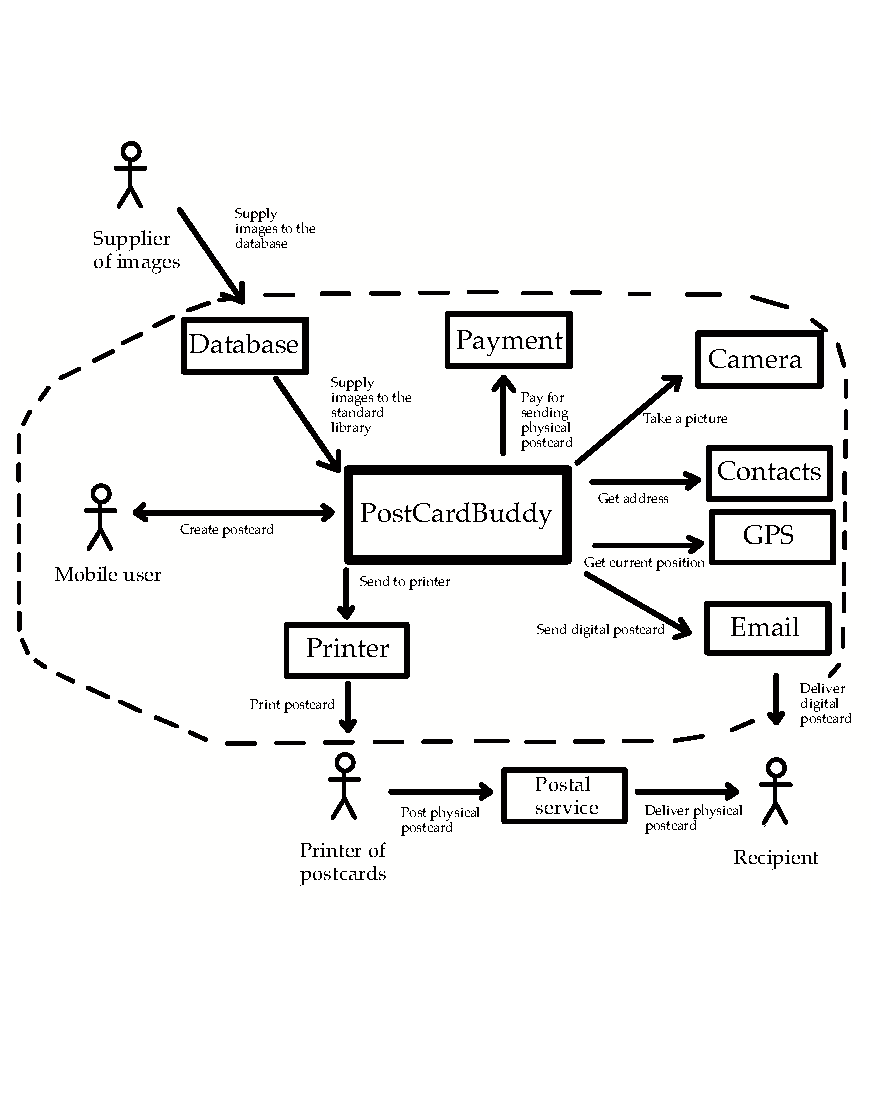
\includegraphics[width=0.7\textwidth]{ContextDiagram4.pdf}
\caption{Context diagram of product.}
\label{fig:context}
\end{figure}
\FloatBarrier

\paragraph{Stakeholders}
Selected stakeholders for PostCardBuddy are presented in Table~\ref{table:stakeholder}. For each stakeholder there is a number to visualize the prioritization. The scale is from 1-5 where 1 represent a high priority and 5 a low priority.


\begin{table}[h!]
\centering
\label{table:deliv}
\begin{tabular}{|l|l|} \hline
\textbf{Stakeholder} & \textbf{Priority} \\
\hline
Mobile user & 1\\
\hline
Printer of postcards & 2\\
\hline
Postal service & 2\\
\hline
Developers & 3\\
\hline
Payment service & 4\\
\hline
The existing application \textit{Riktiga Vykort} & 4\\
\hline

\end{tabular}\\
\caption{Stakeholder prioritization}
\label{table:stakeholder}
\end{table}

\begin{description}
\item[Mobile user] was given the highest priority since they will be the actual users of the product and without them there will be no market.
\item[Printer of postcards] will act as the key customer, since they placed the order of the product, and are thereby given a high priority. 
\item[Postal service] was given a high priority because they are considered a possible buyer of the application in the future. 
\item[Developers] are given a medium priority since they have knowledge about whether a functionality is reasonable or not from a technical perspective.
\item[Payment service] was given a low priority as the payment service will be used only to provide the application with a standardized pay-functionality and is replaceable.
\item[The existing application \textit{Riktiga Vykort}]  is a competitor to the application and has only been used for comparison and is hence given a low priority. 

\end{description}


\paragraph{Tasks}


\begin {description}

\newcounter{tasks}
\stepcounter{tasks}
\item [Req \thesubsubsection {.\thetasks}] The product shall support the following user tasks.

\item[Work area: 1. Vacation] \mbox{}\\
Communicating with friends and family. Usually from a remote location with unreliable internet access. Typically outdoors and overall poor working environment. Simplicity is key to capturing important moments. \newline
Users: Average smart phone user, used to little manual work. 

\item[Work area: 2. Holidays] \mbox{}\\
Communicating with friends and family. Usually in connection to holidays, e.g. Christmas. Personalization and simplicity is important.
 \newline
Users: Average smart phone user, used to little manual work.

\item [Task 1.1] Send a physical postcard.
\begin {description}
\item \textbf{Precondition:} PostcardBuddy is running.

\item \textbf{Sub-tasks:}
\begin{enumerate}
\item Use the camera in the device to take a picture.
\item Allow editing of images.
\item Save images.
\item Add greeting.
\item Add recipients from address book. 
\item Save finished postcard.
\item Preview postcard.
\item Send postcard to printer.
\end{enumerate}

\item \textbf{Variants:}
\begin{itemize}[label={}]
\item[1a] The user selects an image from the personal gallery.
\item[1b] The user selects an image from PostcardBuddy's standard gallery. 
\item[2a] Includes editing of gallery images.
\item[4a] Choose a template greeting.
\item[5a] Manually add address.
\end{itemize}
\end{description}

\item [Task 1.2] Send an E-card.
\begin {description}
\item \textbf{Precondition:} PostcardBuddy is running.

\item \textbf{Sub-tasks:}
\begin{enumerate}
\item Use the camera in the device to take a picture.
\item Allow editing of images.
\item Save images.
\item Add greeting.
\item Save finished postcard.
\item Preview postcard.
\item Send postcard via E-mail.
\end{enumerate}

\item \textbf{Variants:}
\begin{itemize}[label={}]
\item[1a] The user selects an image from the personal gallery.
\item[1b] The user selects an image from PostcardBuddy's standard gallery. 
\item[2a] Includes editing of gallery images.
\item[4a] Choose a template greeting.
\item[7a] Publish postcard on social media.
\end{itemize}
\end{description}

\item [Task 1.3] Send a physical postcard from a saved postcard.
\begin {description}
\item \textbf{Precondition:} PostcardBuddy is running.

\item \textbf{Sub-tasks:}
\begin{enumerate}
\item Load a saved postcard. 
\item Add missing parts to postcard. 
\item Allow editing of postcard.
\item Add recipients from address book. 
\item Preview postcard.
\item Send postcard to printer.
\end{enumerate}

\item \textbf{Variants:}
\begin{itemize}[label={}]

\item[4a] Manually add address.
\end{itemize}
\end{description}


\item [Task 1.4] History

\begin {description}
\item \textbf{Precondition:} PostcardBuddy is running. 

\item \textbf{Sub-tasks:}
\begin{enumerate}
\item View sent postcards and recipients. 
\item Search sent postcards and recipients.

\end{enumerate}
\item \textbf{Variants:}
\begin{itemize}[label={}]

\item[1a] No postcards sent. 
\item[2a] No postcards found for given search criteria. 

\end{itemize}
\end{description}
\end{description}



\paragraph{Interfaces}
Requirements related to the interfaces of the product.

\begin {description}
\newcounter{interf}
\stepcounter{interf}
	\item [Req \thesubsubsection {.\theinterf} Printer] The interface connecting PostCardBuddy and the printed postcards is an off-the-shelf color printer able to handle standard image formats.

\stepcounter{interf}
	\item [Req \thesubsubsection {.\theinterf} Images] Images for the standard gallery will be provided by the supplier of images in JPEG, bnp or png format.

	\stepcounter{interf}
	\item [Req \thesubsubsection {.\theinterf} Data of images] The supplier of images shall tag the image with its GPS coordinates and the system shall be able to handle this data.

\stepcounter{interf}
	\item [Req \thesubsubsection {.\theinterf} Permissions] When users install the application they shall be prompted to grant permission to use the device functionality specified in the context diagram.  
	\begin{description}
\item[Example:] Camera, GPS etc.
	\end{description} 
\end{description}

\subsubsection{Product}
This section describes the functionality at the product level. 
\newcounter{product}
\stepcounter{product}

\paragraph{Images} 
Requirements related to the handling of images and all of them contribute to fulfil goal~\ref{goal:simpl}. Additionally, requirements~\thesubsubsection .1, \thesubsubsection .2 and \thesubsubsection .5 contribute to meet goal~\ref{goal:pers}.	

\begin {description}
\item [Req \thesubsubsection {.\theproduct} Image from phone gallery] It shall be possible to choose pictures from the phone gallery for the front of the postcard.
\stepcounter{product}
\item [Req \thesubsubsection {.\theproduct} Image from camera] It shall be possible to take a picture with the camera within the application and use as image for the front of the postcard. 
\stepcounter{product}
\item [Req \thesubsubsection {.\theproduct} Image from standard gallery] It shall be possible to choose pictures from the standard gallery.
\stepcounter{product}
\item [Req \thesubsubsection {.\theproduct} Image and GPS position] Images from the standard gallery shall be sorted based on the user's GPS position.
\stepcounter{product}
\item [Req \thesubsubsection {.\theproduct} Image editing] The product shall have the following functions for editing images; brightness, contrast, cropping, remove red eyes, filters, pen and text.
\stepcounter{product}
\item [Req \thesubsubsection {.\theproduct} Image saving] It shall be possible to save images to the phone gallery.
\end{description}

\paragraph{Greetings}
Requirements related to greetings, all of them contribute to fulfil goal~\ref{goal:simpl}. Additionally, requirement~\thesubsubsection .7 contributes to meet goal~\ref{goal:pers}.

\stepcounter{product}
\begin{description}
	\item [Req \thesubsubsection {.\theproduct} Greetings] It shall be possible to write greetings within the application.
	\stepcounter{product}
	\item [Req \thesubsubsection {.\theproduct} Auto-generated greetings] It shall be possible to choose a template greeting.
	\stepcounter{product}
	\item [Req \thesubsubsection {.\theproduct} GPS based greetings] The product shall be able to generate greetings based on the GPS position.
	\stepcounter{product}
	\item [Req \thesubsubsection {.\theproduct} Saving greetings] It shall be possible to save a greeting.
	\stepcounter{product}
	\item [Req \thesubsubsection {.\theproduct} Load greetings] It shall be possible to load a saved greeting.
\end{description}

\paragraph{Recipients}
Requirements related to handling of recipients.

\stepcounter{product}
\begin{description}
	\item [Req \thesubsubsection {.\theproduct} Enter recipients] It shall be possible to enter recipients manually.
	\stepcounter{product}
	\item [Req \thesubsubsection {.\theproduct} Phone book recipients] It shall be possible to choose recipients through the contacts of the device.
	\stepcounter{product}
	\item [Req \thesubsubsection {.\theproduct} Multiple recipients] The product shall be able to handle multiple recipients for one postcard.
	\stepcounter{product}
	\item [Req \thesubsubsection {.\theproduct} Favourite recipients] It shall be possible to save recipients as favourites.
	\stepcounter{product}
	\item [Req \thesubsubsection {.\theproduct} Frequent recipients] The product shall show frequently used recipients as favourite recipients.
\end{description}

\paragraph{Postcard}
Requirements related to functionality and handling of the postcard.

\stepcounter{product}
\begin{description}
	\item [Req \thesubsubsection {.\theproduct} Saving postcards] It shall be possible to save postcards.
	\stepcounter{product}
	\item [Req \thesubsubsection {.\theproduct} Reuse postcards] It shall be possible to reuse saved postcards.
	\stepcounter{product}
	
	\item [Req \thesubsubsection {.\theproduct} Preview postcards] It shall be possible to preview postcards before sending it.
	\stepcounter{product}
	
	\item [Req \thesubsubsection {.\theproduct} Digital postcard] It shall be possible to send digital postcards.
	\stepcounter{product}
	\item [Req \thesubsubsection {.\theproduct} Physical postcards] It shall be possible to send physical postcards.
	\stepcounter{product}
	
	\item [Req \thesubsubsection {.\theproduct} Payment] It shall be possible to pay for sending physical postcards.
	\stepcounter{product}
	
	\item [Req \thesubsubsection {.\theproduct} Postcard size] It shall be possible to choose the size of the physical postcard.
	\stepcounter{product}
	\item [Req \thesubsubsection {.\theproduct} Quality of physical postcard] It shall be possible to choose the print quality of physical postcards. 
	\stepcounter{product}
	\item [Req \thesubsubsection {.\theproduct} History] It shall be possible to display the history of sent postcards.
	
	%Ska nedanstående krav vara med?
	\stepcounter{product}
	\item [Req \thesubsubsection {.\theproduct} Social media] Feature for sharing postcards on social media.
\end{description}

\paragraph{Notifications}
Requirements on how to manage notifications.

\begin{description}
\stepcounter{product}
	\item [Req \thesubsubsection {.\theproduct} Success notification] The user shall be notified when an order is sent from a device.
\stepcounter{product}
	\item [Req \thesubsubsection {.\theproduct} Fail notification] The user shall be notified when an order fails to be sent from a device.

\stepcounter{product}
	\item [Req \thesubsubsection {.\theproduct} No internet] If the user places an order on a device that is not connected to the internet, the order shall be stored and sent the next time the device receives internet connection. 
\end{description}

\subsubsection{Design}
This section describes the design and layout of the application and postcards sent from it. 

The images in figure~\ref{fig:prot} are from a prototype and should be used as a guideline rather than as a design requirement.

\newcounter{design}
% Är dethär tillräckligt specifikt? Vill man ha en exempel bild och ett krav som säger att vykortet ska följa formtet?
\begin {description}
\stepcounter{design}
	\item [Req \thesubsubsection {.\thedesign} Front page] The front of the postcard shall be a field containing an image.
\stepcounter{design}
	\item [Req \thesubsubsection {.\thedesign} Text field] The back of the postcard shall contain a text field.
\stepcounter{design}
	\item [Req \thesubsubsection {.\thedesign} Address field] The back of the postcard shall contain an address field.
\stepcounter{design}
	\item [Req \thesubsubsection {.\thedesign} Postage field] The back of the postcard shall contain a postage field. 
\stepcounter{design}
	\item [Req \thesubsubsection {.\thedesign} Postage print] The postage shall be printed in the top right corner on the back of the postcard. 


%ref bug?
\stepcounter{design}
	\item [Req \thesubsubsection {.\thedesign} Start Screen] The application shall start with a screen where it is possible to choose front and back image/text, see figure \ref{fig:p1}.
\stepcounter{design}
	\item [Req \thesubsubsection {.\thedesign} Get image] The application shall let the user choose the image source from a menu, see figure \ref{fig:p2}.
\stepcounter{design}
	\item [Req \thesubsubsection {.\thedesign} Edit image]The application shall give the user a basic image editor to customize the image, see figure \ref{fig:p3}.
\stepcounter{design}
	\item [Req \thesubsubsection {.\thedesign} Recipient address] The application shall have an address input screen with an address-book/contacts (not in image), see figure \ref{fig:p4}.
\end{description}



\begin{figure}[p]
	\centering
	\begin{subfigure}{0.5\textwidth}
		\centering
		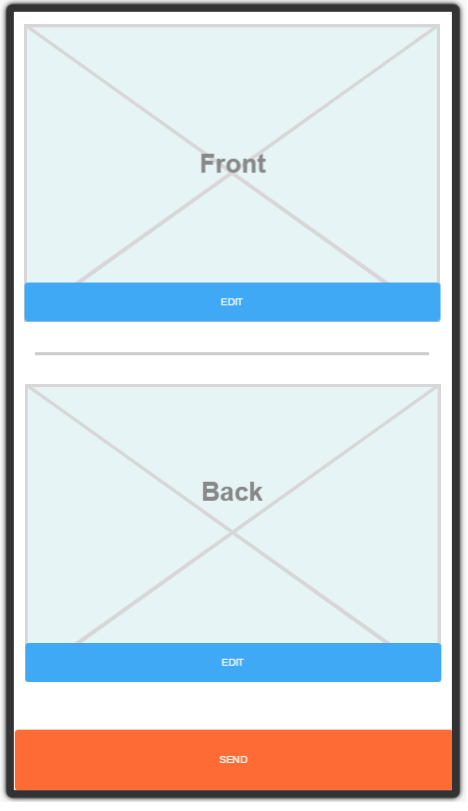
\includegraphics[width=0.5\textwidth]{Prototype_img/p1.png}
		\caption{Start}
		\label{fig:p1}
	\end{subfigure}~
	\begin{subfigure}{0.5\textwidth}
		\centering
		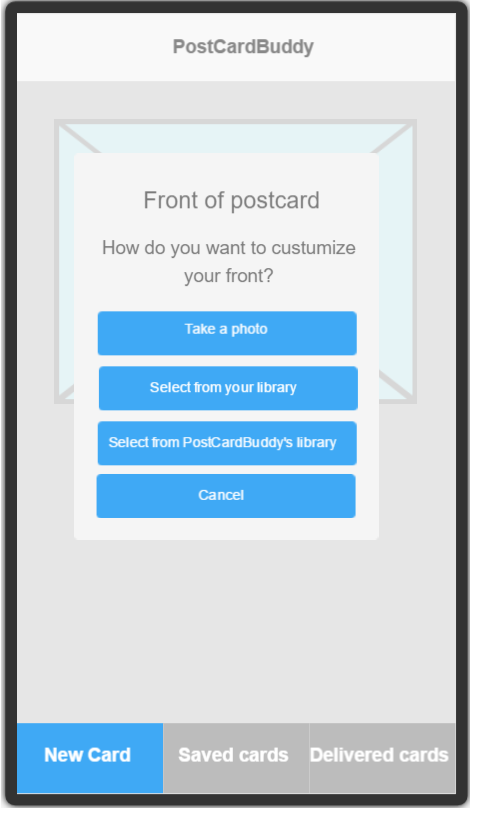
\includegraphics[width=0.5\textwidth]{Prototype_img/p2.png}
		\caption{Choose image source}
		\label{fig:p2}
	\end{subfigure}\\[0.5cm]
	\begin{subfigure}{0.5\textwidth}
		\centering
		
\includegraphics[width=0.5\textwidth]{Prototype_img/p3.png}
		\caption{Image editor}
		\label{fig:p3}
	\end{subfigure}~
	\begin{subfigure}{0.5\textwidth}
		\centering
		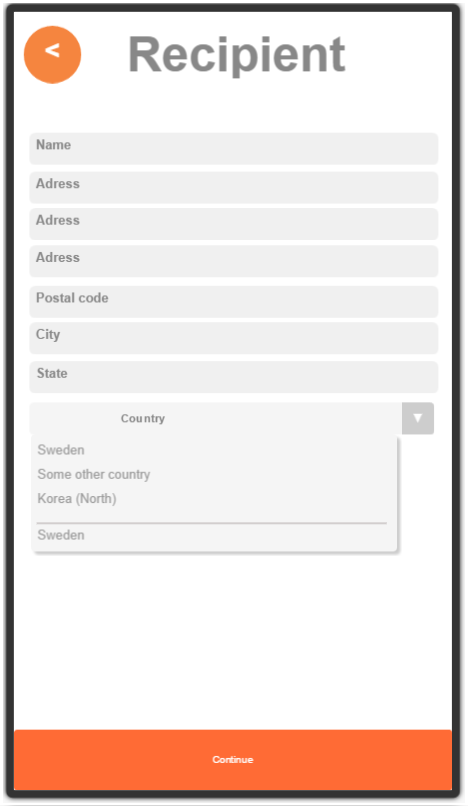
\includegraphics[width=0.5\textwidth]{Prototype_img/p4.png}
		\caption{Recipient information}
		\label{fig:p4}
	\end{subfigure}
	\caption{Example prototype of product.}
	\label{fig:prot}
\end{figure}
\FloatBarrier


	

\subsubsection{Data Requirements}
This section describes the data requirements of the application.

\newcounter{data}

%TODO: Beskrivning till E/R, data dictionary och virtual window när man skapar vykort.
\begin {description}
\stepcounter{data}
	\item [Req \thesubsubsection {.\thedata} Data model] The product shall handle the data presented in the data model in figure \ref{fig:datamodel}.
\end{description}

\begin{figure}[h!]
\centering
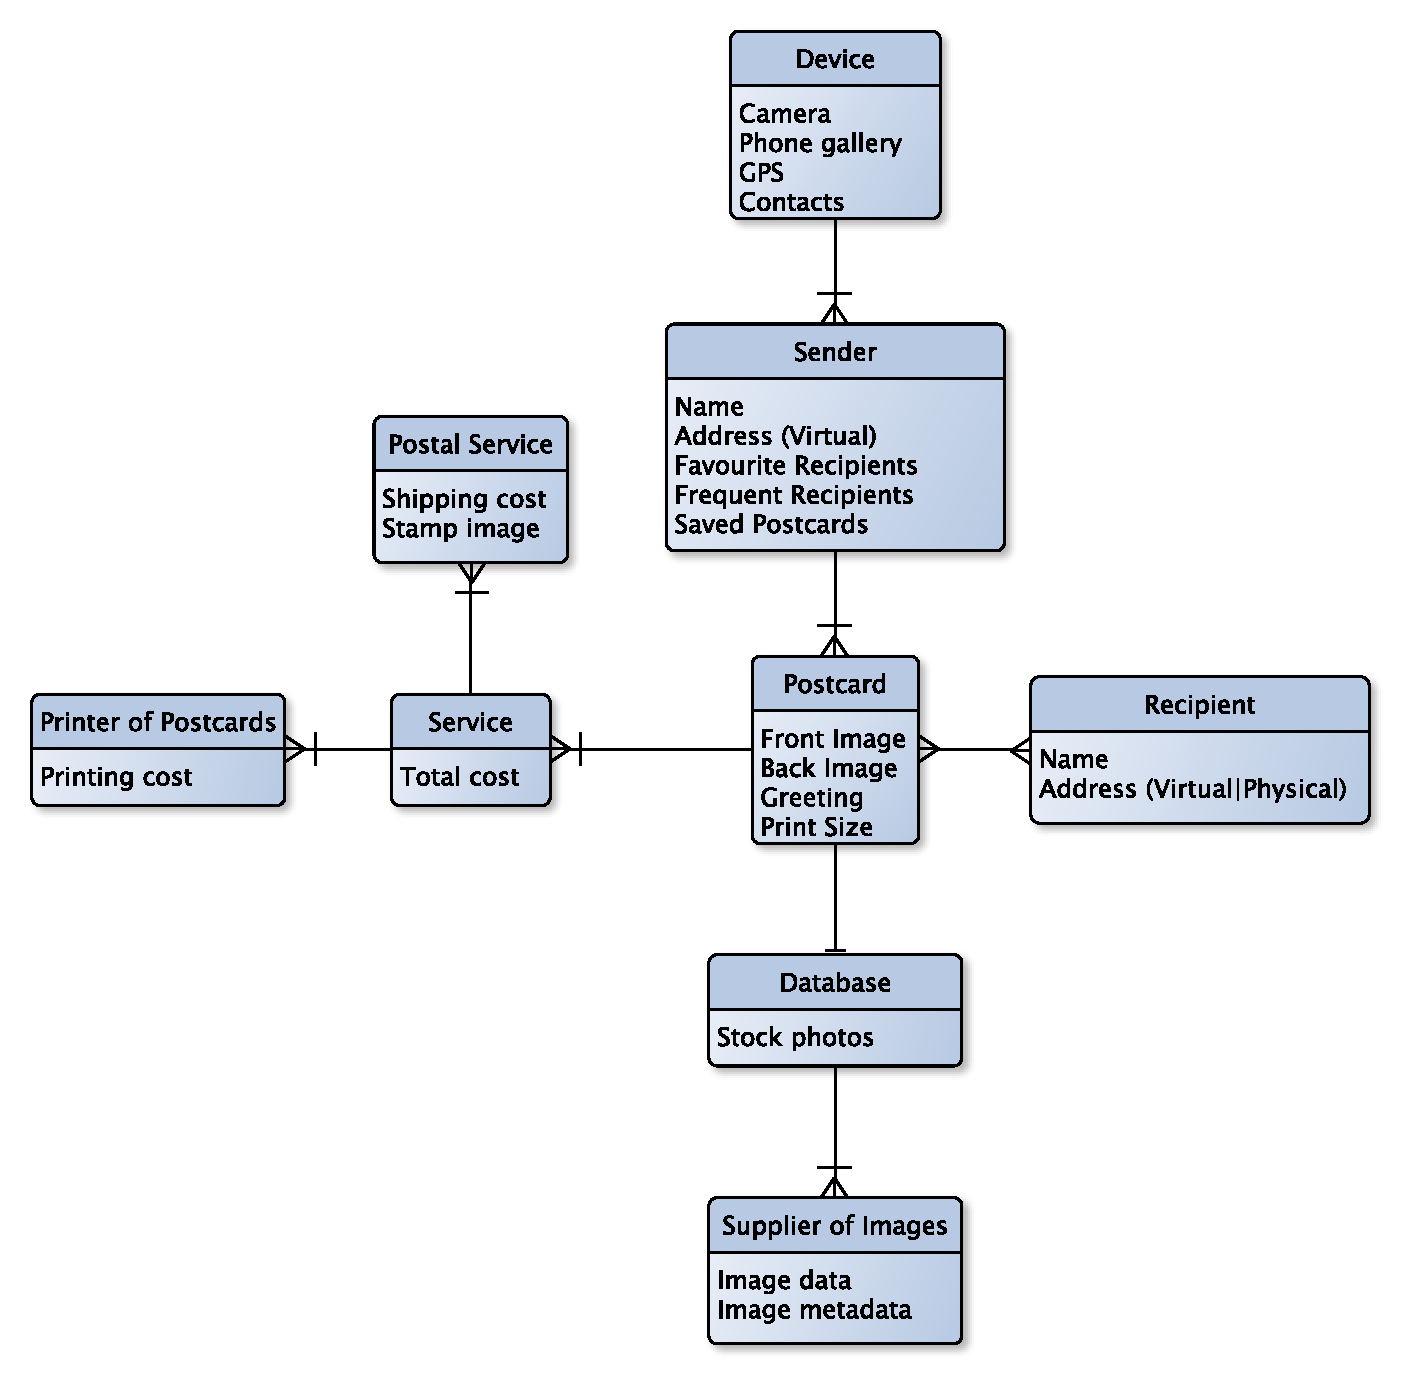
\includegraphics[width=0.7\textwidth]{Data_figures/DataModel.pdf}
\caption{Data model}
\label{fig:datamodel}
\end{figure}
\FloatBarrier
\paragraph{Data dictionary}

%\begin{description}
%\item[Class:] \textbf{Name} \hfill \\
%Description what it is exactly, what it does and what it interacts with
%
%\item[Examples:] \hfill
%\begin{enumerate}
%\item What is this typically?
%\item Special cases.
%\end{enumerate}
%
%\item[Attributes:] \hfill
%\begin{enumerate}
%\item List attributes and 
%\item What type of data it is
%\end{enumerate}
%\end{description}
%
%\hrulefill

%Do we really support both Android and iOS?
\begin{description}
\item[Class:] \textbf{Device} \hfill \\
The device is the actual physical mobile device on which the application is running.

\item[Examples:] \hfill
\begin{enumerate}
\item An android device running the application.
\item An iOS device running the application
\end{enumerate}

\item[Attributes:] \hfill
\begin{enumerate}
\item \textbf{Camera:} Image \hfill \\A compressed image fetched from the devices physical camera.
\item \textbf{GPS:} String[Latitude,longitude] \hfill \\The information about current coordinates from the GPS in the device. The string is given on the format shown and the latitude and longitudes are signed floats with seven decimal places.
\end{enumerate}
\end{description}

\hrulefill

%Maybe we need to divide virtual and physical in separate attributes. Maybe we need data about what platform to share to?
\begin{description}
\item[Class:] \textbf{Sender} \hfill \\
This class represents the person sending the postcard. It can be the same person as the one using the device but it does not have to be.

\item[Examples:] \hfill
\begin{enumerate}
\item The device owner.
\item A person using the application to send a postcard.
\end{enumerate}

\item[Attributes:] \hfill
\begin{enumerate}
\item \textbf{Name:} String \hfill \\The name of the sender. 
\item \textbf{address} (Virtual|Physical): String \hfill \\This attribute is always a string. If it is a virtual address it is a user name, otherwise it is a physical street address. 
\end{enumerate}
\end{description}

\hrulefill

\begin{description}
\item[Class:] \textbf{Recipient} \hfill \\
This class represents the person receiving the postcard. This class is identical to \textit{Sender} in terms of attribute structure. The sender and recipient could be the same person.

\item[Examples:] \hfill
\begin{enumerate}
\item The person receiving the postcard.
\item The same person as the one sending a postcard.
\end{enumerate}
\end{description}

\hrulefill

%Is stamp image required?
\begin{description}
\item[Class:] \textbf{PostCard} \hfill \\
This class represents the postcard sent from the \textit{Sender} to \textit{Recipient}. It encapsulates all the information necessary to send a postcard in either virtual or physical form. An instance of this object, owning a \textit{Sender} and a \textit{Recipient} needs to exist to be able to send a postcard. 

\item[Examples:] \hfill
\begin{enumerate}
\item A postcard with two images, a message and a stamp.
\item A postcard with no images, no message and a stamp.
\item A virtual post card with images, a message and no stamp.
\end{enumerate}

\item[Attributes:] \hfill
\begin{enumerate}
\item \textbf{Front image:} Image [optional] \hfill \\A compressed image that will be used as the front image of the \textit{PostCard}. 
\item \textbf{Back image:} Image [optional] \hfill \\A compressed image that will be used as the back image of the \textit{PostCard}.
\item \textbf{Message:} String [optional] \hfill \\The message on the \textit{PostCard}.
\item \textbf{Stamp image:} Image \hfill \\The image supplied by \textit{Postal service} to properly send the postcard.
\end{enumerate}
\end{description}

\hrulefill

%Maybe we need IDs or names to identify the supplier?
\begin{description}
\item[Class:] \textbf{Suppliers} \hfill \\
This class collects the data from an \textit{Supplier of images}, a \textit{Postal service} and a \textit{Printer of postcards}. 

\item[Examples:] \hfill
\begin{enumerate}
\item A collection of suppliers relevant to printing and sending a specific \textit{PostCard}.
\item Only a printing and shipping cost.
\end{enumerate}

\item[Attributes:] \hfill
\begin{enumerate}
\item \textbf{Total cost:} Float \hfill \\The combined cost of \textit{Supplier of images/Photo cost}, a \textit{Postal service/Shipping cost} and a \textit{Printer of postcards/Printing cost}. The value is rounded up to two decimal places.
\end{enumerate}
\end{description}

\hrulefill

\begin{description}
\item[Class:] \textbf{Supplier of images:} \hfill \\
This class represents a supplier of images. If a user chooses a stock photo as (for example) a \textit{PostCard/Front image} there is a cost with using the photo that needs to be added to the total cost.

\item[Examples:] \hfill
\begin{enumerate}
\item A supplier of images with a photo and a cost.
\item A supplier of images with a free photo.
\end{enumerate}

\item[Attributes:] \hfill
\begin{enumerate}
\item \textbf{Photo cost:} Float \hfill \\The cost of a stock photo. The value is rounded up to two decimal places.
\item \textbf{Stock photo:} Image \hfill \\The actual image that will be bought.
\end{enumerate}
\end{description}

\hrulefill

\begin{description}
\item[Class:] \textbf{Postal service:} \hfill \\
This class represents a postal service. The postal service is the company that will transport the post card. 

\item[Examples:] \hfill
\begin{enumerate}
\item A representation of what is required to send a postcard with Posten.
\item A representation of what is required to send a postcard with DHL.
\end{enumerate}

\item[Attributes:] \hfill
\begin{enumerate}
\item \textbf{Shipping cost:} Float \hfill \\The cost of shipping. The value is rounded up to two decimal places.
\item \textbf{Stock photo:} Image \hfill \\This is the image used on the postcard to indicate that shipping was payed for.
\end{enumerate}
\end{description}

\hrulefill

%Unclear who or what the printer actually is.
\begin{description}
\item[Class:] \textbf{Printer of postcards:} \hfill \\
This class represents a printer. The printer is responsible for printing the physical postcard. 

\item[Examples:] \hfill
\begin{enumerate}
\item A company contracted to print postcards.
\item The company supplying the application.
\end{enumerate}

\item[Attributes:] \hfill
\begin{enumerate}
\item \textbf{Printing cost:} Float \hfill \\The cost of printing. The value is rounded up to two decimal places.
\end{enumerate}
\end{description}


\paragraph{Virtual windows}
Virtual windows displaying data of product can be seen in figure~\ref{fig:vw}.

\begin {description}
\stepcounter{data}
	\item [Req \thesubsubsection {.\thedata} PostCard] The input data to the \textit{PostCard} class described in the data dictionary shall include the items specified in the virtual window in figure \ref{fig:virtualwindows_postcard}.

\stepcounter{data}
	\item [Req \thesubsubsection {.\thedata} Sender] The input data to the \textit{Sender} class described in the data dictionary shall include the items specified in the virtual window in figure \ref{fig:virtualwindows_sender}.

\stepcounter{data}
	\item [Req \thesubsubsection {.\thedata} Recipient] The input data to the \textit{Recipient} class described in the data dictionary shall include the items specified in the virtual window in figure \ref{fig:virtualwindows_recipient}.

\end{description}
\hfill


\begin{figure}[!ht]
\centering
\begin{subfigure}{0.3\textwidth}
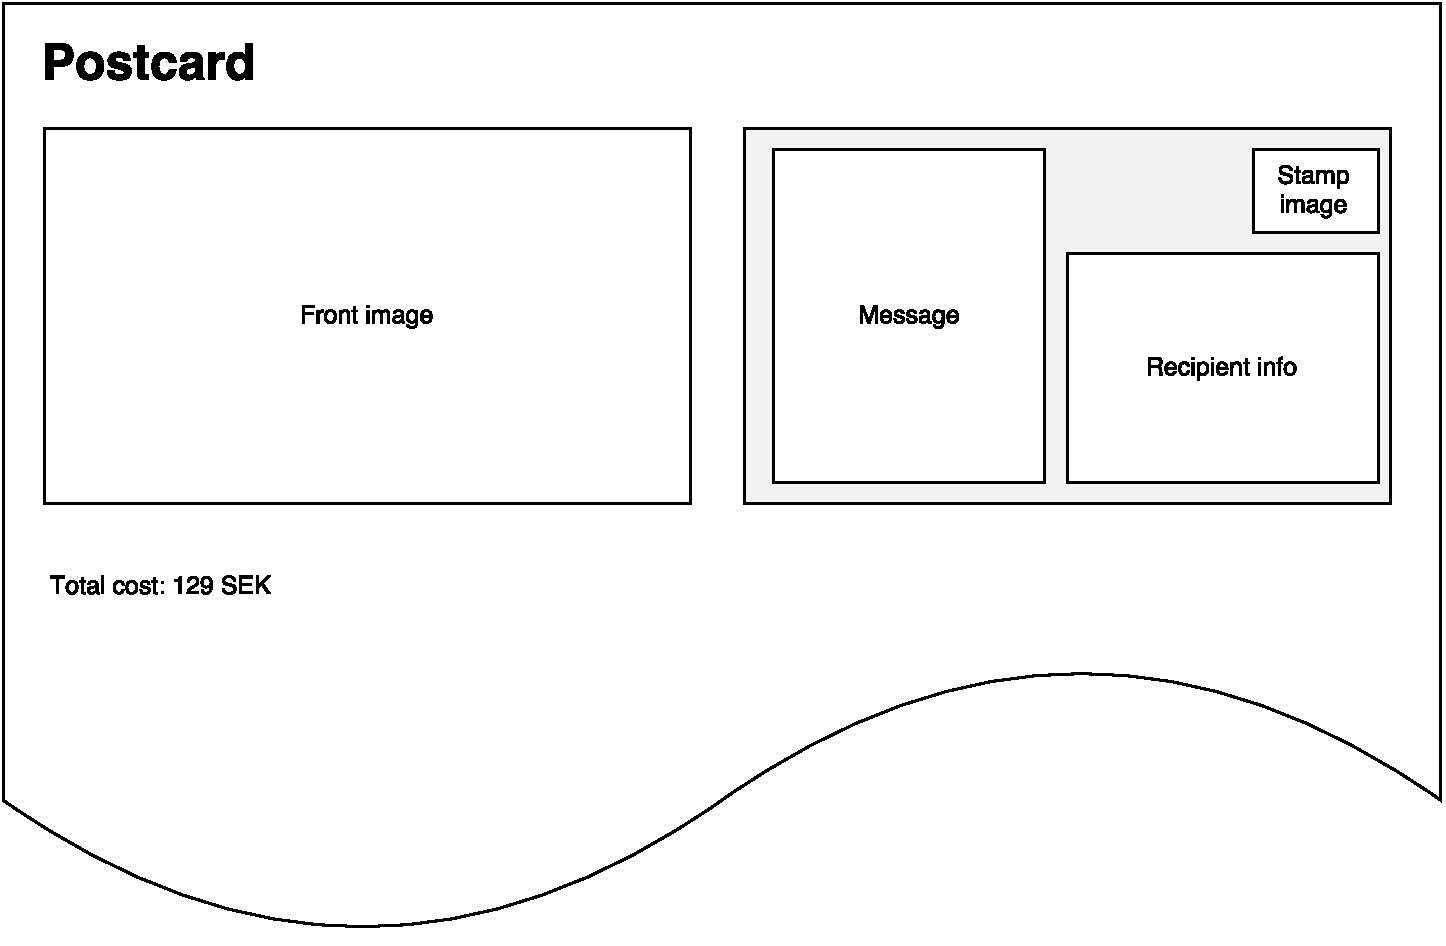
\includegraphics[width=\linewidth]{Data_figures/virtualwindows_postcard.pdf}
\caption{PostCard}
\label{fig:virtualwindows_postcard}
\end{subfigure}\hfill
~
\begin{subfigure}{0.3\textwidth}
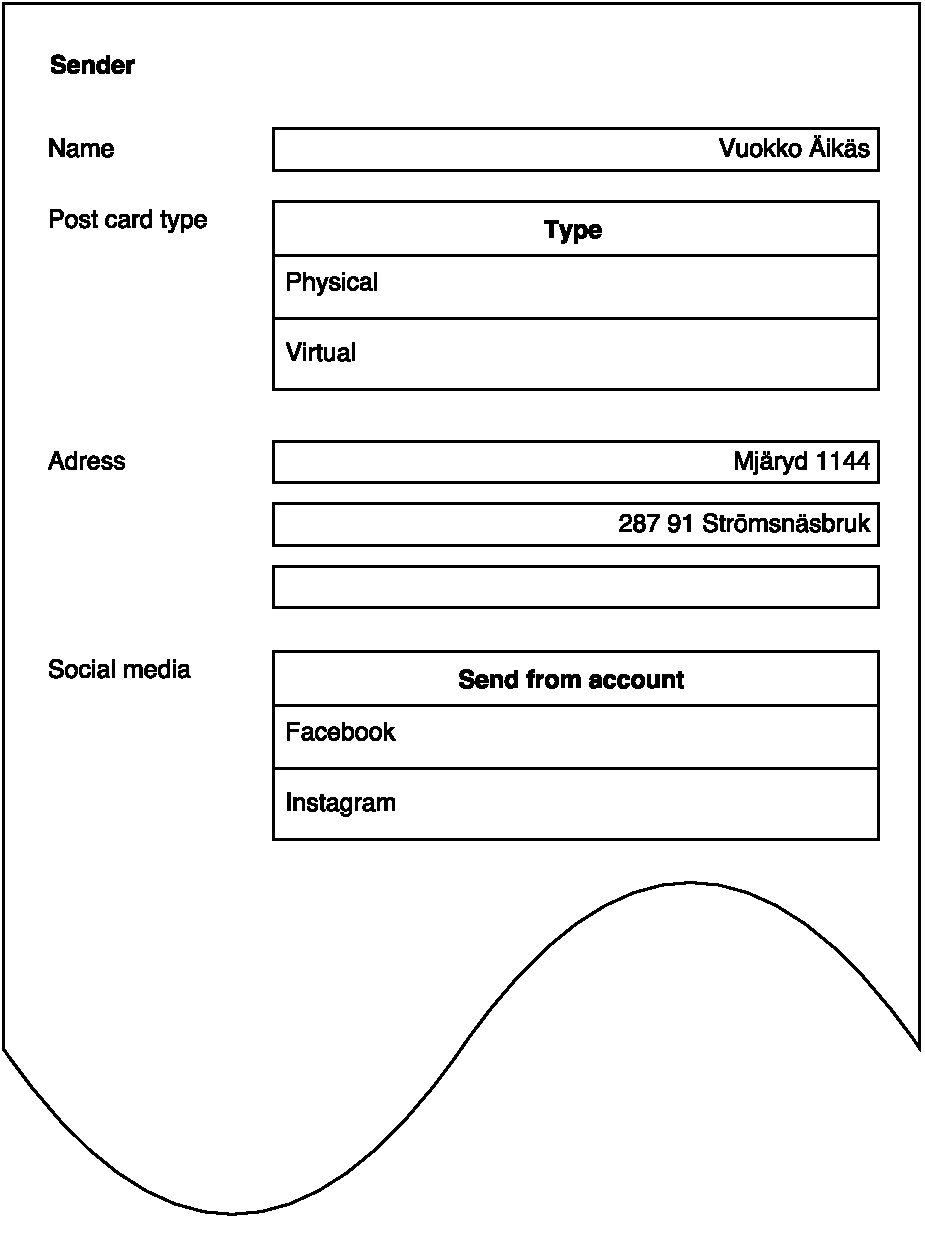
\includegraphics[width=\linewidth]{Data_figures/virtualwindows_sender.pdf}
\caption{Sender}
\label{fig:virtualwindows_sender}
\end{subfigure}\hfill
~
\begin{subfigure}{0.3\textwidth}
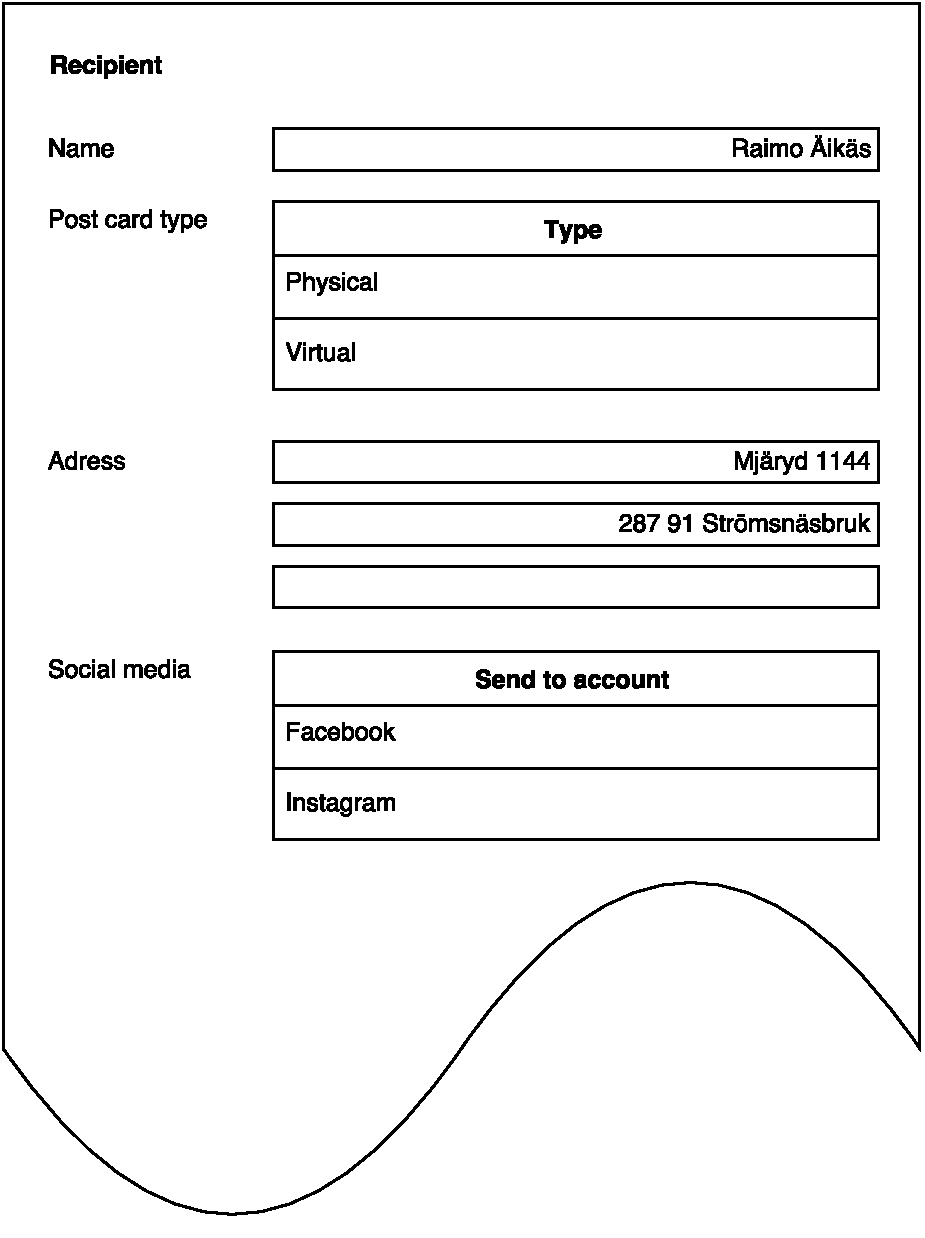
\includegraphics[width=\linewidth]{Data_figures/virtualwindows_recipient.pdf}
\caption{Recipient}
\label{fig:virtualwindows_recipient}
\end{subfigure}
\caption{Virtual windows displaying data of product.}
\label{fig:vw}

\end{figure}



\subsection{Quality Requirements}



\subsubsection{Quality grid}
This quality grid seen in table~\ref{tab:qg} highlights quality factors for certain identified elements. Elements not in the grid can be seen as having status "As usual". Numbers in the quality grid are references to the numbers below the grid. The "x" does not have a reference.

\begin{table}[h!]
	\centering
	\caption{Quality grid}
	\label{tab:qg}
	\begin{tabular}{|l|l|l|l|l|l|}
		\hline
		\textbf{\begin{tabular}[c]{@{}l@{}}Quality factors -\\ PostCardBuddy\end{tabular}} & \textbf{Critical} & \textbf{Important} & \textbf{As usual} & \textbf{Unimportant} & \textbf{Ignore} \\ \hline
		\textbf{Operation}                                                                 &                   &                    &                   &                      &                 \\ \hline
		Integrity/Security                                                                 &                   &                    & 1                 &                      &                 \\ \hline
		Reliability/availability                                                           &                   & 2                  &                   &                      &                 \\ \hline
		Usability                                                                          & 3                 &                    &                   &                      &                 \\ \hline
		Internet connection demand                                                         & 4                 &                    &                   &                      &                 \\ \hline

		\textbf{Miscellaneous}                                                             &                   &                    &                   &                      &                 \\ \hline
		Installability                                                                     &                   & 5                  &                   &                      &                 \\ \hline
		Interoperability                                                                   &                   & 6                  &                   &                      &                 \\ \hline
	\end{tabular}
\end{table}

\begin{enumerate}
\item PostCardBuddy uses an integrated payment solution for sending physical postcards. Integrity/Security shall be as usual for an application that contains an integrated payment solution.
\item Many users may use PostCardBuddy when they are on vacation. Therefore it is important the application will work in a wide geographical area while still being reliable. Users sending digital, or physical, postcards not coming through will not be pleased.
\item The standard user might just send a few postcards a year. Because of this it is critical that the application is easy to use. Users should not need to go through unnecessary menus and steps. It should be quick and easy to create a postcard and press "send".
\item Internet connection when on vacation is often a problem. It is therefore critical that PostCardBuddy has a low internet demand. Some users might only use PostCardBuddy on their vacation.
\item Users may install PostCardBuddy while on their vacation. Internet connection might be weak and disconnects from internet could be common. Also users might need to leave internet zones for trips on their vacation.
\item PostCardBuddy saves files to the smartphone and uses features as the phone's camera and gallery.
\end{enumerate}

\subsubsection{QUPER}
A quper diagram takes into consideration quality and performance. This specific quper diagram measures time to get access to a specific image, from standard gallery, reference figure~\ref{fig:quper}.


\begin{figure}[h!]
\centering
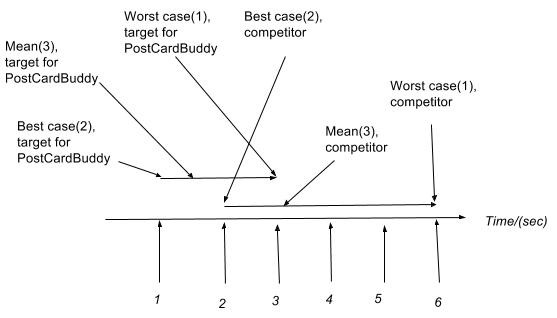
\includegraphics[width=0.7\textwidth]{QUPER_v1.jpg}
\caption{Time measured from requesting access to a specific image in the standard gallery to it being loaded in to creating a postcard. For the competitor this was done ten times with different pictures. 
Competitor, "Riktiga Vykort", was measured with a OnePlus One smartphone. The targeted area for PostCardBuddy should be done with the same kind of smartphone and tested in as a similar way as possible.\newline
(1) Longest time measured. (2) Shortest time measured (3) The mean of the test. }
\label{fig:quper}
\end{figure}


\subsubsection{Performance}
All performance requirements shall be fulfilled on a Nexus~5/iPhone~5 running original firmware without any other user installed applications on the phone. Background tasks should be kept at a minimal by closing applications before testing.

\newcounter{perf}
\begin{description}
	\stepcounter{perf}
	\item [Req \thesubsubsection {.\theperf} Application size] The installed size of the application excluding user data shall not exceed 30MB.	
	\stepcounter{perf}
	\item [Req \thesubsubsection {.\theperf} Speed] The user interface shall respond within 200~ms after a finished user interaction if there should be an response. The test shall be done so that the above values can be guaranteed within a 95\% confidence interval.
	\stepcounter{perf}
	\item [Req \thesubsubsection {.\theperf} Memory] The application shall use less than 200MB RAM when editing a 8MP image. This is tested by using the all tools after each other which is one iteration. It passes the test if it can do 50 iterations without finishing the edit and uses less than 200MB RAM in the process.
	\stepcounter{perf}
	\item [Req \thesubsubsection {.\theperf} Picture quality] The camera shall be able to take a picture in the highest hardware supported resolution. This requirement also applies to the latest iPhone/Nexus at the time of release for the application e.g. iPhone 6S (plus) and Nexus 6P/5X at 10/12/15.
	\stepcounter{perf}
	\item [Req \thesubsubsection {.\theperf} Autofocus] The camera shall have an autofocus that is comparable to the Android/iOS stock camera. This means that the time to focus can't take longer than 0.5 sec more than the stock camera and the focus plane distance must be within 20\% of the stock camera if the stock distance is less than 10m. The motive should be light and have good contrast to support for this requirement. The test shall be done so that the above values can be guaranteed within a 95\% confidence interval.
\end{description}

\subsubsection{Maintainability/Portability}
Maintainability and portability of product.
\newcounter{mapo}
\begin{description}
	\stepcounter{mapo}
	\item [Req \thesubsubsection {.\themapo} Language] The application shall be developed in non-native language e.g. Java for Android. 
	\stepcounter{mapo}
	\item [Req \thesubsubsection {.\themapo} Device support] The application shall work on devices with operating systems Android~4.1/iOS~7.0.1 or newer.
\end{description}

\subsubsection{Usability}
Usability of product.
\newcounter{usab}
\begin{description}
	\stepcounter{usab}
	\item [Req \thesubsubsection {.\theusab} User friendly] 9 out of 10 users shall be able to use the application after a five minute instruction.
\end{description}





%--------------------------------------------------------------------%
%--------------- Specification Techniques ---------------------------%
%--------------------------------------------------------------------%
% Several different specification techniques (e.g. context diagrams, features, virtual windows, task descriptions).

% 3A) apply more than one suitable specification technique (e.g. task descriptions and screen prototypes)
% 4B) use at least four different specification techniques adequately tailored to the context.
% 3B) define a system’s boundaries and its interaction with external entities.
% 5A) combine specification techniques in an explicitly motivated trade off between qualities and costs, where a high degree of specification completeness is achieved for a carefully selected subset of requirements.
% 5C) go beyond initial stakeholders and given frames, while challenging the domain boundaries and eliciting creative ideas and deep domain knowledge in real-world contexts.


%--------------------------------------------------------------------%
%------------------ Release Plan ------------------------------------%
%--------------------------------------------------------------------%
% A release plan defining which requirements that are implemented in each of three releases, namely R3 (final release for this course project), and the imagined future releases R4 and R5. The release plan shall include information used to derive the plan such as priorities and cost.
% The requirements planned for R3 (in the release plan) should be implemented as mock-up designs (e.g. screens and prototypes, analog drawings, clickable presentations, executable gui mockups) and thus included in the final (R3) release.

% 4H) create a release plan for a subset of prioritized features, while taking into account precedence constraints.
% 5F) combine priorities from several stakeholders and use priorities and scheduling constraints to iteratively create a relevant release plan.
\section{Release Plan}

\begin{table}[h!]
\centering
\label{table:release}
\begin{tabular}{| l | l | l | } \hline
\textbf{Release} & \textbf{Functionality} & \textbf{cost [h]} \\ \hline
1 & Greeting & 6\\ \hline
1 & Physical postcard & 120\\ \hline
1 & Image from phone gallery & 15\\ \hline
1 & Payment & 150\\ \hline
1 & Picture from camera & 24\\ \hline
1 & Enter recipients & 15\\ \hline
2 & Image and GPS position & 15\\ \hline
2 & Preview postcards & 30\\ \hline
2 & Multiple recipients & 15\\ \hline
2 & Image from standard library & 90\\ \hline
2 & Phone book recipients & 15\\ \hline
2 & Auto-generated greetings & 15\\ \hline
2 & Handwritten greetings on screen & 15\\ \hline
2 & Pictures of handwritten greetings & 30\\ \hline
3 &  Favorite recipients & 9\\ \hline
3 & Frequent recipients & 9\\ \hline
3 & Quality of physical postcard & 9\\ \hline
3 & Postcard size & 24\\ \hline
3 & History & 15\\ \hline
3 & Image diting & 150\\ \hline
3 & Saving postcards & 15\\ \hline
3 & Reuse postcards & 30\\ \hline
3 & Image saving & 9\\ \hline
3 & GPS based greetings &15\\ \hline
3 & Saving greetings & 9\\ \hline
3 & Digital postcard &15\\ \hline
3 & Social media &15\\ \hline
\end{tabular}\\
\caption{Release plan}
\end{table}


\begin{table}[h!]
\centering
\label{table:SumRelease}
\begin{tabular}{| l | l |} \hline
\textbf{Release} & \textbf{total sum [h]} \\ \hline

1 &  330 \\ \hline
2 & 225 \\ \hline
3 & 324 \\ \hline
\end{tabular}\\
\caption{Summary of the cost for each release}
\end{table}


\end{document}

